\section{Methods}
\label{sec:methods}

Fig.~\ref{fig:arch} summarizes the pipeline shared by all experiments. Every
experiment is defined by one YAML file that inherits from a common base
configuration, so runs differ only in the factors listed in
Table~\ref{tab:protocol}.

\begin{figure*}[t]
  \centering
  \resizebox{\textwidth}{!}{% Architecture diagram (fig:arch). Self-contained tikzpicture: needs tikz with
% libraries arrows.meta, positioning, fit, backgrounds, calc.
% Included by main.tex (scaled to \textwidth) and by architecture_standalone.tex (PNG export).
\begin{tikzpicture}[
  font=\footnotesize,
  >={Stealth[length=2.2mm]},
  flow/.style={->, thick, draw=black!75},
  skip/.style={->, thick, draw=orange!80!black},
  lowskip/.style={->, thick, draw=violet!80!black},
  box/.style={draw=black!70, rounded corners=2pt, align=center, inner sep=3pt},
  enc/.style={box, draw=blue!55!black, fill=blue!10, minimum width=3.0cm, minimum height=0.62cm, font=\scriptsize},
  encdim/.style={enc, draw=blue!30, fill=blue!4, text=black!55},
  udec/.style={box, draw=orange!75!black, fill=orange!12, minimum width=2.9cm, minimum height=0.62cm, font=\scriptsize},
  ddec/.style={box, draw=violet!75!black, fill=violet!10, minimum height=0.62cm, font=\scriptsize},
  head/.style={box, draw=black!60, fill=black!6, minimum height=0.62cm, font=\scriptsize},
  panel/.style={draw=black!35, rounded corners=4pt, inner sep=6pt},
  ptitle/.style={font=\small\bfseries, anchor=south west},
  lbl/.style={font=\scriptsize, text=black!70},
]

% =====================================================================
% TOP: shared pipeline
% =====================================================================
\begin{scope}[yshift=0.45cm]
  % Input "image" icon: sky / tree line / trail.
  \begin{scope}[shift={(0,-0.75)}]
    \fill[blue!30] (0,0.95) rectangle (1.8,1.5);
    \fill[green!45!black!70] (0,0.55) -- (0.3,1.05) -- (0.55,0.8) -- (0.85,1.15) -- (1.15,0.85) -- (1.45,1.1) -- (1.8,0.8) -- (1.8,0.55) -- cycle;
    \fill[green!55!black!45] (0,0) rectangle (1.8,0.58);
    \fill[brown!55] (0.6,0) -- (0.85,0.58) -- (0.98,0.58) -- (1.35,0) -- cycle;
    \draw[black!70] (0,0) rectangle (1.8,1.5);
  \end{scope}
  \node[lbl, align=center, anchor=north] (inlbl) at (0.9,-0.8) {RGB input\\$3\times384\times384$\\ImageNet-normalized};
  \coordinate (inR) at (1.8,0);

  % Encoder trapezoid (wide input side, narrow deep side).
  \draw[draw=blue!55!black, fill=blue!10, rounded corners=1pt]
    (3.0,-1.1) -- (3.0,1.1) -- (5.75,0.6) -- (5.75,-0.6) -- cycle;
  \coordinate (encW) at (3.0,0); \coordinate (encE) at (5.75,0);
  \node[align=center, font=\footnotesize, inner sep=0pt] (enc) at (4.3,0) {\textbf{Encoder}\\ResNet-18 / -50\\ImageNet init.\\{\scriptsize features $\tfrac12\ldots\tfrac1{32}$}};
  \draw[flow] (inR) -- (encW);

  % Decoder choices.
  \node[udec, minimum width=3.1cm, font=\footnotesize] (dU) at (8.55,0.52) {\textbf{(a) U-Net decoder}\\skips at every scale};
  \node[ddec, minimum width=3.1cm, font=\footnotesize] (dD) at (8.55,-0.62) {\textbf{(b) DeepLabV3+ decoder}\\ASPP @ $\tfrac1{16}$ + skip @ $\tfrac14$};
  \node[lbl, font=\scriptsize\itshape] at (8.55,-0.05) {or};
  \node[draw=black!40, dashed, rounded corners=3pt, fit=(dU)(dD), inner sep=3pt] (dec) {};
  \draw[flow] (encE) -- (encE -| dec.west);

  % Logits.
  \node[head, minimum width=2.1cm, minimum height=1.0cm, font=\footnotesize] (logit) at (12.0,0) {\textbf{Logits}\\$25\times384\times384$};
  \draw[flow] (dec.east) -- (logit.west);

  % Training loss and evaluation.
  \node[box, draw=red!60!black, fill=red!6, text width=4.15cm, font=\scriptsize, anchor=west] (loss) at (13.75,0.5)
    {\textbf{Training loss} (one per run)\\CE $\cdot$ weighted CE (median-freq.)\\Dice $\cdot$ Focal ($\gamma{=}2$) $\cdot$ CE+Dice\\void pixels ignored};
  \node[box, draw=green!45!black, fill=green!7, text width=4.15cm, font=\scriptsize, anchor=west] (eval) at (13.75,-0.72)
    {\textbf{Evaluation}: argmax (void masked)\\per-class IoU, mIoU, 6-group IoU};
  \draw[flow] (logit.east) -- ++(0.25,0) |- (loss.west);
  \draw[flow] (logit.east) -- ++(0.25,0) |- (eval.west);
\end{scope}

% =====================================================================
% Shared helper geometry for the two detail panels.
%   rows: y(1/1)=-2.75, y(1/2)=-3.5, y(1/4)=-4.25, y(1/8)=-5.0, y(1/16)=-5.75, y(1/32)=-6.5
% =====================================================================
\def\yA{-2.75}\def\yB{-3.5}\def\yC{-4.25}\def\yD{-5.0}\def\yE{-5.75}\def\yF{-6.5}

% =====================================================================
% BOTTOM LEFT: (a) U-Net
% =====================================================================
\begin{scope}[xshift=0cm]
  \node[lbl] (uin) at (1.6,\yA) {input $384^2$};
  \node[enc] (u1) at (1.6,\yB) {stem\enspace$\tfrac12$\enspace 64 | 64};
  \node[enc] (u2) at (1.6,\yC) {layer1\enspace$\tfrac14$\enspace 64 | 256};
  \node[enc] (u3) at (1.6,\yD) {layer2\enspace$\tfrac18$\enspace 128 | 512};
  \node[enc] (u4) at (1.6,\yE) {layer3\enspace$\tfrac1{16}$\enspace 256 | 1024};
  \node[enc] (u5) at (1.6,\yF) {layer4\enspace$\tfrac1{32}$\enspace 512 | 2048};
  \foreach \a/\b in {uin/u1,u1/u2,u2/u3,u3/u4,u4/u5} \draw[flow] (\a) -- (\b);

  \node[udec] (ud1) at (6.45,\yE) {up$\times$2, concat, 2$\times$conv\enspace 256};
  \node[udec] (ud2) at (6.45,\yD) {up$\times$2, concat, 2$\times$conv\enspace 128};
  \node[udec] (ud3) at (6.45,\yC) {up$\times$2, concat, 2$\times$conv\enspace 64};
  \node[udec] (ud4) at (6.45,\yB) {up$\times$2, concat, 2$\times$conv\enspace 32};
  \node[udec] (ud5) at (6.45,\yA) {up$\times$2, 2$\times$conv\enspace 16};
  \foreach \a/\b in {ud1/ud2,ud2/ud3,ud3/ud4,ud4/ud5} \draw[flow] (\a) -- (\b);
  \draw[flow] (u5.east) -| (ud1.south);

  \foreach \e/\d in {u1/ud4,u2/ud3,u3/ud2,u4/ud1} \draw[skip] (\e.east) -- (\d.west);
  \node[lbl, text=orange!70!black, anchor=north] at ($(u4.east)!0.5!(ud1.west)+(0,-0.03)$) {skips};

  \node[head] (uh) at (9.45,\yA) {3$\times$3 conv\\$\to$ 25};
  \draw[flow] (ud5) -- (uh);
\end{scope}
\node[panel, fit=(uin)(u5)(ud5)(uh)(ud1)] (pa) {};
\node[ptitle] at (pa.north west) {(a) U-Net};

% =====================================================================
% BOTTOM RIGHT: (b) DeepLabV3+
% =====================================================================
\begin{scope}[xshift=11.0cm]
  \node[lbl] (din) at (1.6,\yA) {input $384^2$};
  \node[encdim] (d1) at (1.6,\yB) {stem\enspace$\tfrac12$\enspace 64 | 64};
  \node[enc] (d2) at (1.6,\yC) {layer1\enspace$\tfrac14$\enspace 64 | 256};
  \node[encdim] (d3) at (1.6,\yD) {layer2\enspace$\tfrac18$\enspace 128 | 512};
  \node[encdim] (d4) at (1.6,\yE) {layer3\enspace$\tfrac1{16}$\enspace 256 | 1024};
  \node[enc] (d5) at (1.6,\yF) {layer4\enspace$\tfrac1{16}$ (dilated)\enspace 512 | 2048};
  \foreach \a/\b in {din/d1,d1/d2,d2/d3,d3/d4,d4/d5} \draw[flow] (\a) -- (\b);

  \node[ddec, text width=2.3cm, anchor=west] (aspp) at (4.4,\yF)
    {\textbf{ASPP} @ $\tfrac1{16}$: 1$\times$1, rates 12/24/36, image pool $\to$ 256};
  \draw[flow] (d5.east) -- (aspp.west);

  \node[ddec, anchor=west] (low) at (4.4,\yC) {1$\times$1 conv\enspace 48};
  \draw[lowskip] (d2.east) -- (low.west);
  \node[lbl, text=violet!75!black, anchor=south] at ($(d2.east)!0.5!(low.west)+(0,0.05)$) {skip};

  \node[ddec, text width=1.35cm, anchor=west] (fuse) at (6.7,\yC) {concat, 3$\times$3 sep.\ conv 256};
  \draw[flow] (low.east) -- (fuse.west);
  \draw[flow] (aspp.east) -| node[pos=0.75, lbl, right, align=left] (uplbl) {bilinear\\up$\times$4\\($\tfrac1{16}\!\to\!\tfrac14$)} (fuse.south);

  \node[head] (dh) at (fuse.north |- 0,\yA) {1$\times$1 conv $\to$ 25, up$\times$4};
  \draw[flow] (fuse.north) -- (dh.south);
\end{scope}
\node[panel, fit=(din)(d5)(aspp)(dh)(fuse)(uplbl)] (pb) {};
\node[ptitle] at (pb.north west) {(b) DeepLabV3+};

% Legend line under the panels.
\node[lbl, anchor=north west, font=\scriptsize] at ($(pa.west |- pb.south)+(0,-0.08)$)
  {Encoder blocks: name, resolution, output channels for ResNet-18 | ResNet-50. Pale blocks: computed but not used by the decoder.};
\end{tikzpicture}
}
  \caption{Shared segmentation pipeline. Top: a $384\times384$ RGB frame is
  encoded by an ImageNet-pretrained ResNet-18 or ResNet-50, decoded by U-Net
  or DeepLabV3+, and mapped to 25 logits per pixel (24 RUGD classes plus
  \emph{void}, which is ignored in the loss and never predicted). Each
  experiment trains with exactly one loss variant. Bottom left: the U-Net
  decoder concatenates encoder features at every scale from $1/16$ to $1/2$.
  Bottom right: DeepLabV3+ dilates the last ResNet stage (output stride 16),
  applies ASPP, and fuses the result with a single $1/4$-scale skip connection.
  Channel counts are given for ResNet-18 / ResNet-50.}
  \label{fig:arch}
\end{figure*}

\subsection{Data and Splits}
\label{sec:data}

RUGD~\cite{wigness2019rugd} provides 7,436 annotated $688\times550$ frames from
18 video sequences. We use the official sequence-level split
(Table~\ref{tab:data}): no sequence appears in more than one split, so
near-identical consecutive frames cannot leak from training into evaluation. The
sequence assignment matches Table~I of~\cite{wigness2019rugd}. A split-check
script counts 4,779\,/\,733\,/\,1,924 frames in the released data. The paper's
table prints 4,759 and 1,964 for train and test, which sum to 20 more frames than
the 7,436 released. We use the counts from the released files.

\begin{table}[t]
  \centering
  \caption{RUGD sequence-level split used in all experiments.}
  \label{tab:data}
  \footnotesize
  \begin{tabular}{@{}l p{4.3cm} r@{}}
    \toprule
    Split & Sequences & Frames \\
    \midrule
    Train & park-2, trail, trail-3, -4, -6, -9, -10, -11, -12, -14, -15, village & 4,779 \\
    Val   & park-8, trail-5 & 733 \\
    Test  & creek, park-1, trail-7, trail-13 & 1,924 \\
    \bottomrule
  \end{tabular}
\end{table}

\textbf{Label decoding.} RUGD labels are color-coded RGB images. We decode them
to integer class indices with a 24-bit color lookup table built from the
dataset's own colormap file (25 entries: \emph{void} plus 24 classes). Any
color not in the table maps to an ignore index. \emph{Void} pixels are also
mapped to the ignore index, so they contribute to neither loss nor metrics, and
the void logit is masked out at prediction time.

\textbf{Class statistics.} Pixel frequencies on the training split
(Fig.~\ref{fig:classfreq}) span almost four orders of magnitude, from
\emph{tree} (39.3\% of labeled pixels) to \emph{sign} (0.006\%). Two
properties of the split affect evaluation directly. First, \emph{bridge} has
zero training pixels but about 4.6\,M test pixels. Second, the validation split
contains no \emph{sand}, \emph{rock-bed}, \emph{bicycle}, or \emph{bridge}
pixels, and the test split contains no \emph{bicycle} pixels (consistent with
Table~IV of~\cite{wigness2019rugd}).

\begin{figure}[t]
  \centering
  % Class pixel frequency on the RUGD TRAINING split (non-void pixels), log scale.
% Data: results/class_freq_rugd.csv (scripts/compute_class_weights.py).
% bridge (0 training pixels) cannot be drawn on a log axis and is noted in the caption.
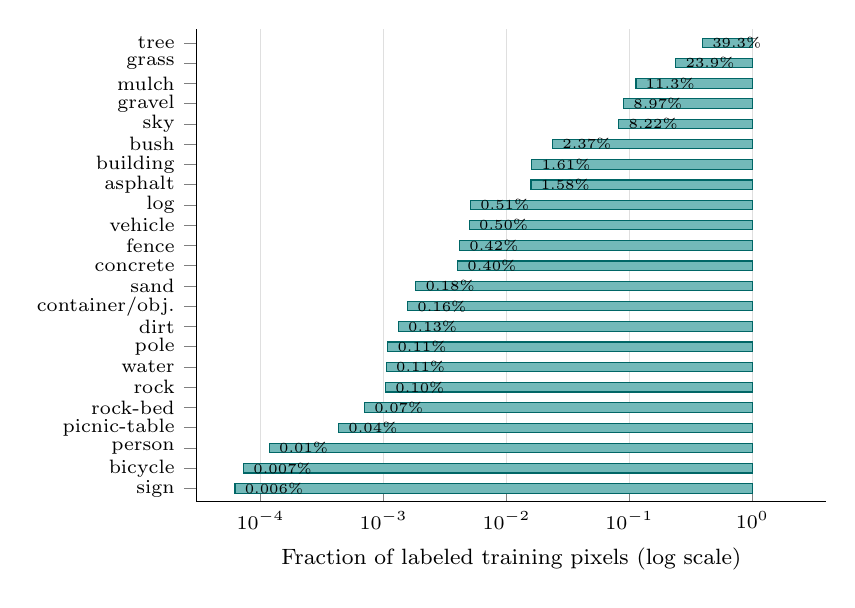
\begin{tikzpicture}
\begin{axis}[
  xbar,
  scale only axis,
  width=0.66\linewidth,
  height=6.0cm,
  bar width=3.4pt,
  xmode=log,
  log basis x=10,
  xmin=3e-5, xmax=4,
  xtick={1e-4,1e-3,1e-2,1e-1,1},
  xlabel={Fraction of labeled training pixels (log scale)},
  xlabel style={font=\footnotesize},
  symbolic y coords={sign,bicycle,person,picnic-table,rock-bed,rock,water,pole,dirt,container/obj.,sand,concrete,fence,vehicle,log,asphalt,building,bush,sky,gravel,mulch,grass,tree},
  ytick=data,
  y tick label style={font=\scriptsize},
  x tick label style={font=\scriptsize},
  enlarge y limits=0.03,
  axis x line*=bottom,
  axis y line*=left,
  xmajorgrids,
  grid style={gray!25},
  nodes near coords,
  nodes near coords style={font=\tiny, anchor=west, /pgf/number format/.cd, fixed, precision=2},
  point meta=explicit symbolic,
]
\addplot[fill=teal!55, draw=teal!80!black] coordinates {
  (0.393337,tree)       [39.3\%]
  (0.238506,grass)      [23.9\%]
  (0.113075,mulch)      [11.3\%]
  (0.089696,gravel)     [8.97\%]
  (0.082180,sky)        [8.22\%]
  (0.023742,bush)       [2.37\%]
  (0.016065,building)   [1.61\%]
  (0.015838,asphalt)    [1.58\%]
  (0.005103,log)        [0.51\%]
  (0.004991,vehicle)    [0.50\%]
  (0.004165,fence)      [0.42\%]
  (0.004008,concrete)   [0.40\%]
  (0.001836,sand)       [0.18\%]
  (0.001570,container/obj.) [0.16\%]
  (0.001322,dirt)       [0.13\%]
  (0.001083,pole)       [0.11\%]
  (0.001056,water)      [0.11\%]
  (0.001041,rock)       [0.10\%]
  (0.000701,rock-bed)   [0.07\%]
  (0.000432,picnic-table) [0.04\%]
  (0.000118,person)     [0.01\%]
  (0.000073,bicycle)    [0.007\%]
  (0.000062,sign)       [0.006\%]
};
\end{axis}
\end{tikzpicture}

  \caption{Class pixel frequency on the RUGD training split (void excluded,
  log scale). \emph{Bridge} has no training pixels and is not shown. The two
  most frequent classes cover 63\% of labeled pixels, while the
  safety-relevant \emph{water}, \emph{rock}, and \emph{log} together cover
  0.72\%.}
  \label{fig:classfreq}
\end{figure}

\subsection{Preprocessing and Augmentation}

Images are normalized with ImageNet channel statistics to match the pretrained
encoders. All transforms use Albumentations~\cite{buslaev2020albumentations};
images are interpolated bilinearly and masks with nearest neighbor, so labels
are never blended. For training, we apply a random resized crop covering
50--100\% of the frame area with aspect ratio 0.75--1.33, resized to
$384\times384$; a horizontal flip ($p=0.5$); brightness and contrast jitter of
$\pm0.3$ ($p=0.7$), which approximates the shift between deep shade and harsh
sun; and a hue/saturation/value shift of $\pm5/\pm20/\pm10$ ($p=0.3$). We do not
use vertical flips, because the sky is always at the top of the frame. For
validation and test, the full frame is resized to $384\times384$ without
cropping. This slightly compresses the 1.25:1 frame horizontally. All metrics are
computed at this resolution against nearest-neighbor-resized labels.

\subsection{Models}

Both architectures come from the Segmentation Models PyTorch library
(v0.6.0)~\cite{iakubovskii2019smp} on PyTorch~\cite{paszke2019pytorch}, with
ResNet encoders~\cite{he2016resnet} initialized from ImageNet
weights~\cite{deng2009imagenet} unless stated otherwise (E8).

\textbf{U-Net}~\cite{ronneberger2015unet}: five decoder blocks, each of which
upsamples by $2\times$, concatenates the encoder feature map of matching
resolution ($1/16$, $1/8$, $1/4$, $1/2$; the last block has no skip), and
applies two $3\times3$ convolutions with batch normalization. Decoder widths are
256, 128, 64, 32, and 16 channels, followed by a $3\times3$ convolution to 25
logits at full resolution.

\textbf{DeepLabV3+}~\cite{chen2018deeplabv3plus}: the last ResNet stage is
dilated so that the deepest features stay at output stride 16. ASPP applies
depthwise-separable atrous convolutions at rates 12, 24, and 36, a $1\times1$
convolution, and image-level pooling, with 256 channels and dropout of
0.5~\cite{chen2017deeplabv3}. The result is upsampled $4\times$ and concatenated
with the $1/4$-scale encoder features, reduced to 48 channels by a $1\times1$
convolution. A separable $3\times3$ convolution fuses them, and a $1\times1$
head with $4\times$ bilinear upsampling produces the 25 logits.

\subsection{Loss Functions}
\label{sec:losses}

Let $\Omega$ be the set of non-void pixels in a mini-batch, $y_i$ the label of
pixel $i$, $z_{i,c}$ its logits, $p_{i,c}=\mathrm{softmax}_c(z_i)$, and
$g_{i,c}=\mathbb{1}[y_i=c]$. The number of output classes is $C=25$.

\textbf{Cross-entropy (CE)}:
$\mathcal{L}_\mathrm{CE} = -\frac{1}{|\Omega|}\sum_{i\in\Omega}\log p_{i,y_i}$.

\textbf{Weighted CE} (normalized as in PyTorch):
\begin{equation}
  \mathcal{L}_\mathrm{wCE} =
  -\frac{\sum_{i\in\Omega} w_{y_i}\log p_{i,y_i}}{\sum_{i\in\Omega} w_{y_i}},
  \label{eq:wce}
\end{equation}
\begin{equation}
  w_c = \min\!\Big(\frac{\operatorname{median}_k f_k}{f_c},\,50\Big),
  \label{eq:mfw}
\end{equation}
where $f_c$ is the fraction of labeled \emph{training} pixels belonging to class
$c$, the median is taken over classes present in training, and classes absent
from training (\emph{void}, \emph{bridge}) get $w_c=0$. This is a variant of
median-frequency balancing~\cite{eigen2015predicting}: Eigen and Fergus compute
$f_c$ only over images that contain class $c$, whereas we use the global pixel
fraction. Weights are computed from the training split alone and range from
0.010 (\emph{tree}) to the clip value of 50, which is reached by \emph{bicycle}
and \emph{sign} (\emph{person}: 34.1). The median class is \emph{concrete}
($w=1$). The clip keeps a handful of pixels from dominating a batch.

\textbf{Dice}~\cite{milletari2016vnet}, computed over the whole batch for each
class:
\begin{equation}
  \mathcal{L}_\mathrm{Dice} = \frac{1}{C}\sum_{c=1}^{C} \delta_c
  \Big(1-\frac{2\sum_{i\in\Omega}p_{i,c}g_{i,c}}
  {\sum_{i\in\Omega}p_{i,c}+\sum_{i\in\Omega}g_{i,c}+\epsilon}\Big),
\end{equation}
with $\delta_c=\mathbb{1}[\sum_i g_{i,c}>0]$ (classes absent from the batch
contribute zero) and $\epsilon=10^{-7}$.

\textbf{Focal}~\cite{lin2017focal}, $\gamma=2$, no $\alpha$ balancing. As in the
library implementation, it is applied one-vs-rest with sigmoid probabilities
$q_{i,c}=\sigma(z_{i,c})$ and averaged over classes:
\begin{equation}
  \mathcal{L}_\mathrm{Focal} = \frac{1}{C}\sum_{c=1}^{C}\frac{1}{|\Omega|}
  \sum_{i\in\Omega} -(1-q^{t}_{i,c})^{\gamma}\log q^{t}_{i,c},
\end{equation}
where $q^{t}_{i,c}=q_{i,c}$ if $g_{i,c}=1$ and $1-q_{i,c}$ otherwise.

\textbf{CE+Dice}: $\mathcal{L}=\mathcal{L}_\mathrm{CE}+\mathcal{L}_\mathrm{Dice}$
(unweighted CE, equal coefficients).

\subsection{Optimization}

All runs use AdamW~\cite{loshchilov2019adamw} with learning rate
$3\times10^{-4}$, weight decay $10^{-4}$, and batch size 8 (597 iterations per
epoch, last partial batch dropped) for 25 epochs (14,925 steps). The learning
rate warms up linearly over the first 200 steps and then follows a per-step
cosine decay to zero~\cite{loshchilov2017sgdr}. After every epoch we compute
validation mIoU, and the checkpoint with the highest validation mIoU (not the
last one) is used for all reported evaluations. The default seed is 0. Training
can resume from a per-epoch checkpoint.

\subsection{Evaluation Metrics}
\label{sec:metrics}

We accumulate a $25\times25$ confusion matrix over all non-void pixels of a
split and compute per-class IoU, $\mathrm{IoU}_c =
\mathrm{TP}_c/(\mathrm{TP}_c+\mathrm{FP}_c+\mathrm{FN}_c)$. \textbf{mIoU}
averages IoU over classes that occur in the ground truth or the predictions,
excluding \emph{void} and \emph{bridge}. We exclude \emph{bridge} because it has
no training pixels, so no method trained on this split can learn it, and every
published RUGD baseline scores 0.0 on it~\cite{wigness2019rugd}. Including it
would lower every model's mIoU by the same structural amount and say nothing
about the methods. We still report its per-class IoU, and the evaluation code
also outputs mIoU with \emph{bridge} included. A class that is absent from a
split's ground truth but is predicted (\eg\emph{bicycle} on test) enters the
mean with IoU 0, which penalizes false positives. \textbf{Pixel accuracy} is the
fraction of non-void pixels classified correctly.

\textbf{Traversability groups.} To measure errors that matter for driving, and
to enable the RELLIS-3D test, we also map both predictions and labels to six
groups (Table~\ref{tab:groups}) and report group IoU and group mIoU. This is
coarser than GA-Nav's grouping~\cite{guan2022ganav} and was fixed before any
results were seen.

\begin{table}[t]
  \centering
  \caption{Six-group traversability map used for group IoU and the RELLIS-3D test.}
  \label{tab:groups}
  \footnotesize
  \begin{tabular}{@{}l p{3.0cm} p{2.6cm}@{}}
    \toprule
    Group & RUGD classes & RELLIS-3D classes \\
    \midrule
    Smooth ground & dirt, sand, asphalt, concrete, mulch & dirt, asphalt, concrete \\
    Rough ground  & gravel, rock-bed & mud, rubble \\
    Vegetation    & grass, bush & grass, bush \\
    Water         & water & water, puddle \\
    Obstacle      & tree, pole, vehicle, container, building, log, bicycle, person, fence, sign, rock, bridge, picnic-table
                  & tree, pole, vehicle, object, building, log, person, fence, barrier \\
    Sky           & sky & sky \\
    \bottomrule
  \end{tabular}
\end{table}

\subsection{Experimental Protocol}
\label{sec:protocol}

Table~\ref{tab:protocol} lists the experiments. Each changes one factor
relative to its reference. An orchestration script runs the whole matrix and
makes every model-selection decision automatically from \emph{validation} mIoU,
logging each decision to a JSON file:
(1)~E0 must reach at least 0.70 mIoU on its own 50-image training subset,
otherwise the pipeline is considered broken and the run stops;
(2)~the better of E2 and E3 becomes the architecture for E4--E8;
(3)~the best loss is chosen among the CE winner of E2/E3 and E4--E7;
(4)~E8 combines the best architecture and loss with randomly initialized
weights;
(5)~the two best configurations among E1--E7 are retrained with seeds 1 and 2,
which gives three seeds each (E9).
The test split is used only by the evaluation script, which refuses to run on
it without an explicit confirmation flag. It is evaluated once per final
configuration, after all selection is complete.

\begin{table}[t]
  \centering
  \caption{Experiment matrix. All runs: $384^2$, 25 epochs, batch 8, AdamW.
  ``Best'' choices are made automatically from validation mIoU.
  $^\ast$Random initialization.}
  \label{tab:protocol}
  \footnotesize
  \setlength{\tabcolsep}{3pt}
  \begin{tabular}{@{}l l l l p{2.35cm}@{}}
    \toprule
    ID & Arch. & Enc. & Loss & Question \\
    \midrule
    E0 & U-Net & R18 & CE & Overfit 50 images? \\
    E1 & U-Net & R18 & CE & Baseline \\
    E2 & U-Net & R50 & CE & Encoder depth (vs.\ E1) \\
    E3 & DLV3+ & R50 & CE & Decoder (vs.\ E2) \\
    E4 & best & R50 & wCE & Class reweighting \\
    E5 & best & R50 & Dice & Overlap loss \\
    E6 & best & R50 & Focal & Hard pixels \\
    E7 & best & R50 & CE+Dice & Combined loss \\
    E8 & best & R50$^\ast$ & best & ImageNet init.\ value \\
    E9 & \multicolumn{3}{l}{top-2 of E1--E7, seeds 0/1/2} & Seed variance \\
    \bottomrule
  \end{tabular}
\end{table}

\subsection{Compute and Deviations from the Proposal}
\label{sec:compute}

All training runs on a single Apple M1 Pro laptop GPU (PyTorch MPS backend,
16\,GB unified memory). Our proposal planned $512\times512$ inputs and about 50
epochs on Colab-class GPUs with mixed precision. Benchmarking DeepLabV3+/ResNet-50
on our hardware gave about 0.64\,s per batch of 8 at $384^2$ versus about
1.2\,s at $512^2$, and mixed precision gave no speedup on MPS. At $384^2$, a
25-epoch DeepLabV3+/ResNet-50 run takes about 2.7\,h of training steps
alone. To fit the 14 planned runs into our schedule, we
therefore train at $384^2$ for 25 epochs in full FP32 precision (the code
enables mixed precision only on CUDA). This is a deliberate deviation from the
proposal. It reduces the effective resolution of thin structures such as poles,
signs, and log edges, and it may leave models slightly under-trained. Both
effects apply equally to all compared configurations. E8 (random
initialization) uses the same schedule as the pretrained runs, so it measures
the benefit of pretraining under a fixed budget rather than at convergence.
